\documentclass[journal,12pt,twocolumn]{IEEEtran}
\usepackage[utf8]{inputenc}
\usepackage{graphicx}
\usepackage{amssymb}
\usepackage{amsmath}
\title{Assignment 1}
\author{Kotikalapudi Karthik \\
CS21BTECH11030}

\begin{document}

\maketitle

\textbf{ICSE class 10 2018}\\
\textbf{Question 9(c)}\\
The following figure represents a solid consisting of a right circular cylinder with a hemisphere at one end and cone at the other. Their common radius is $7cm$. The height of the cylinder and the cone are each of $4cm$. Find the volume of the solid.\\
\begin{figure}[ht!]
	  \centering 
	  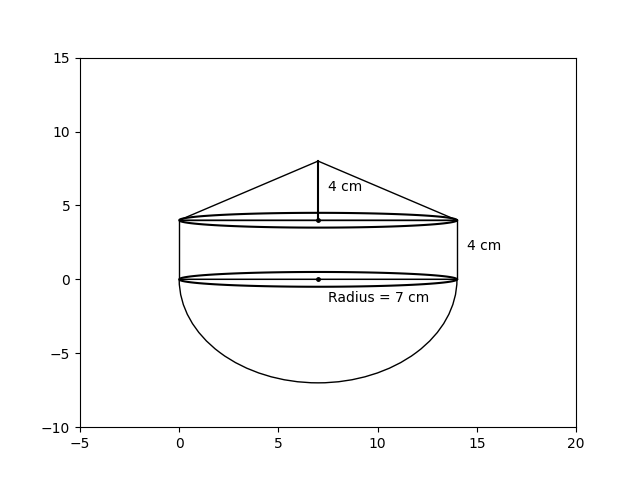
\includegraphics[width=\columnwidth]{Figs/Diagram.png}
	  \caption{Solid}
\end{figure}

\textbf{Steps for generating the figure:}
\begin{enumerate}
    \item Construct a cylinder with height $4cm$ and radius $7cm$.
    \item Then, construct a cone of height $4cm$ such that its circular surface is having radius $7cm$ and coinciding with top surface of the cylinder.
    \item In the same way, construct a hemisphere coinciding with the other circular surface of cylinder with radius $7cm$.
    \item Therefore, the required figure is generated.
\end{enumerate}
\textbf{Solution :}\\
The various parameters considered in this problem are listed in Table
\eqref{table:Table1}
\\
\begin{table}[ht!]
    \centering
    
\begin{tabular}{|c|c|c|}
\hline
 Symbol & Value & Description \\
\hline
 $r$  & $7cm$  & radius of cone, cylinder and hemisphere  \\
 \hline
 $h$  & $4cm$  & height of cone and cylinder  \\
\hline
$V1$ & $\frac{1}{3} \pi r^2 h$ & Volume of cone\\
\hline
$V2$ & $\pi r^2 h$ & Volume of cylinder\\
\hline
$V3$ & $\frac{1}{3} \pi r^3$ & Volume of hemisphere\\
\hline
$V$ & ? & Volume of the figure\\
\hline
\end{tabular}
    \caption{}
    \label{table:Table1}
\end{table}

From the given information, the volume of the figure is equal to the sum of the volume of the cone, cylinder and hemisphere. Thus,
\begin{align*}
    V &= V_1 + V_2 + V_3\\
    \implies V &= \frac{1}{3} \pi r^2 h + \pi r^2 h + \frac{2}{3} \pi r^3
    \\
    \therefore V&= \frac{2}{3} \pi r^2 (2h+r)
    \\
    \text{By substituting $h$ and $r$,}
    \\
    V &= \frac{2}{3} \times 49 (8+7) \pi
    \\
    &= 490 \pi
    \\ 
    &\approx 1539.38cm^3
\end{align*}
\end{document}
